\chapter{Informação mútua, teoria de cópulas e dependência estatística}
\section{Dependência Estatística e medidas de dependência}


\newthought{O conceito de dependência estatística} é central à teoria de probabilidades. Fazer hipóteses a respeito da dependência estatística entre as variáveis de interesse em um modelo é comum em diversas áreas -- da física à análise financeira. Não é óbvio, entretanto, como expressar esse conceito de maneira precisa. A formalização precisa desse conceito é um dos objetivos desse capítulo. De maneira informal e grosseira, dependência estatística diz respeito a quanta \textit{informação} se obtém a respeito de uma variável quando o valor de outra variável é conhecido. Os dois casos extremos podem ser mais facilmente entendidos em primeira análise: o caso de completa independência e o caso de completa dependência. Duas variáveis são ditas independentes se sua distribuição conjunta pode ser fatorada em um produto\footnote{Manteremos o foco de nossa atenção em distribuições bivariadas, uma vez que a generalização é imediata.}:
\begin{equation}
\label{eq:independence}
 p_{X,Y}(x,y) = p_{X}(x)p_{Y}(y).
\end{equation}
De maneira similar, pode-se dizer que duas variáveis são independentes quando a distribuição condicional $p(x|y)$ é idêntica à distribuição marginal de $X$ - $p_{X}(x)$. Nessa situação, o conhecimento do valor da variável $Y$ não fornece qualquer informação a respeito da variável $X$. Duas variáveis são ditas completamente dependentes quando uma pode ser escrita como função monotônica da outra:
\begin{equation}
x = F(y).
\end{equation}
Nesse caso, o conhecimento de uma das variáveis determina completamente o valor de outra. Ou seja $p(x | y)  = \delta(x - F(y))$, com $F(\cdot)$ uma função monotônica. Pode-se, dessa maneira, tentar introduzir alguma forma concreta de medir a dependência estatística em um parâmetro que possa ser estimado e usado para caracterizar a dependência entre variáveis de forma mais concreta.

\newthought{Um parâmetro comumente usado} para esse fim é a chamada correlação linear\footnote{A rigor, o módulo da correlação linear. A correlação linear mede, além de dependência, concordância, ou seja, quanto duas variáveis reais apresentam variação coordenada de seus sinais. Essa informação extra não é captada apenas pelo conceito de dependência.}
\begin{equation}
 \hat{\rho}_{XY} = \frac{\E{XY} - \E{X}\E{Y}}{\sigma_X \sigma_Y} = \frac{\mathrm{Cov}(X,Y)}{\sigma_X \sigma_Y}.
\end{equation}
A correlação linear $\hat{\rho}$ é um número real no intervalo $[-1,1]$, simétrica com relação à transposição de X e Y que sempre se anula quando duas variáveis são independentes. É certamente a medida mais popular de dependência utilizada em todo tipo de análise estatística. Entretanto, seria mais preciso dizer que a correlação linear, como a nomenclatura aqui empregada sugere, é apenas uma medida de dependência linear. Há diversas falhas dessa medida em capturar a completa dependência entre duas variáveis. Em particular é fácil notar que é possível obter duas variavéis com correlação linear nula em que, entretanto, haja forte dependência entre ambas. Um exemplo simples é o par de variáveis definido por:
\begin{equation}
 Y = f(X) + \epsilon
\end{equation}
em que X e $\epsilon$ sejam independentes e tenham distribuições simétricas em torno da origem e $f(\cdot)$ seja qualquer função par. Nesse caso temos:
\begin{equation*}
 \mathrm{Cov}(X,Y) = E[X f(X)] + E[X] E[\epsilon] - E[X] E[f(X)]
\end{equation*}
Note que se a distribuição de X é uma função par, então o valor esperado de qualquer função ímpar de X é nulo, o que anula a expressão acima. Dessa forma temos $\hat{\rho}_{XY} = 0$. Entretanto, caso a distribuição de $\epsilon$ seja bastante concentrada em torno da origem, o conhecimento de $X$ pode fornecer informação quase completa a respeito de $Y$. Essa informação não é capturada pela correlação linear. O epíteto ``linear'', usado nesse trabalho para descrever a correlação, pode ser melhor compreendido se notarmos uma propriedade interessante da correlação: ela é invariante por mudanças de escala lineares nas variáveis X e Y. Uma reparametrização do tipo:
\begin{align*}
 X' &= \alpha_{X} X + \beta_{X} \\
 Y' &= \alpha_{Y} Y + \beta_{Y} 
\end{align*}
não muda o valor da correlação linear: $\hat{\rho}_{X'Y'} = \hat{\rho}_{XY}$. Entretanto uma mudança mais geral de escala não preserva essa propriedade. Uma  nova variável:
\begin{equation*}
Y' = g(Y)
\end{equation*}
com $g(\cdot)$ monotônica, a princípio contém exatamente a mesma informação a respeito de $X$ que a antiga variável $Y$. Entretanto não se garante que a correlação se mantenha invariante. Seria esperado, além disso, que a afirmação de que a correlação entre duas variáveis é máxima em módulo fosse uma indicação de que a dependência entre as duas variáveis é máxima. Entretanto, isso não é garantido. 

\subsection{O que se deseja de uma medida de dependência?}

\newthought{A digressão acima} acerca da natureza da correlação linear imediatamente suscita a pergunta: que parâmetros são boas medidas de dependência e quais são suas características? Pode-se enumerar uma série de desejos a respeito dessas medidas que se baseiem na noção intuitiva de dependência como o conteúdo de informação de uma variável a respeito de outra. Explicitamente, esperamos que:
\begin{enumerate}
\item \label{item:funcional} uma boa medida de dependência seja um funcional $R : P_{2} \to \mathbb{R}$ da distribuição conjunta de probabilidades, bem definido para qualquer par de variáveis aleatórias X e Y; 
\item \label{item:simétrico} o funcional seja invariante sob permutação das variávies X e Y: $R(X,Y) = R(Y,X)$;
\item \label{item:indep} o funcional seja nulo \textit{se, e somente se} as variáveis forem estritamente independentes;
\item \label{item:maximo} o funcional atinja um valor máximo \textit{se, e somente se} as variáveis apresentem dependência máxima, ou seja, sejam funções monotônicas uma da outra;
\item \label{item:invariante} o funcional seja invariante por escolhas de novas variáveis $(X, Y) \rightarrow (U = u(X), V = v(Y))$ desde que nenhuma informação seja perdida, ou seja, desde que  $u(\cdot)$ e $v(\cdot)$ sejam funções bijetoras;
\item \label{item:normal} o funcional seja uma função monotônica e crescente do módulo da correlação linear para o caso de distribuições conjuntas gaussianas.	
\end{enumerate}
Essa série de requisitos, essencialmente\footnote{Rényi exigia ainda que a medida tomasse valores no conjunto $[0,1]$, o que dispensamos, uma vez que é sempre possível transpor uma medida no intervalo $[0,\infty]$ para esse conjunto através de uma função monotônica. Além disso há requisitos de continuidade e convergência para sequências convergentes de distribuições.} enumerados pela primeira vez \cite{Renyi1959, schweizer1981} por \citet{Renyi1959} , não são suficientes para escolher um parâmetro único e são satisfeitos por uma grande variedade de diferentes parâmetros usados em estatística. Como exemplo podemos citar o $\tau$ de Kendall. Dados dois pares, $(X_1, Y_1)$ e $(X_2,Y_2)$, de pontos sorteados independentemente da distribuição $p_{XY}(x,y)$, o $\tau$ de Kendall é dado por:
\begin{align*}
 \tau_{XY} &= \Prob{(X1-X2)(Y1 - Y2) > 0} - \Prob{(X1-X2)(Y1 - Y2) < 0} \\
      &= 4 \int F(x,y) dF(x,y) - 1  , 
\end{align*}
 onde $F(x,y)$ é a distribuição cumulativa de $X$ e $Y$. Outra medida que satisfaz esses requisitos é a correlação de postos de Spearman dada por:
\begin{align}
 \rho^{S}_{XY} = 12 \int \left(F(x,y) - F_{X}(x)F_Y(y)\right) dF_X(x) dF_Y(y),
\end{align}
onde $F_X(x)$ e $F_Y(y)$ são as distribuições cumulativas marginais de $X$ e $Y$ respectivamente. 

\section{Informação Mútua}
\newthought{Do ponto de vista de teoria de informação} a dependência mútua de um conjunto de variáveis pode ser quantificada através da mínima ``distância na variedade estatística'' (divergência de Kullback-Leibler) entre a distribuição conjunta dessas variáveis e a ``sub-variedade'' de distribuições independentes (veja figura \ref{fig:distributionmanyfold}) Isso pode ser escrito da forma:
\begin{figure}
	\centering
    	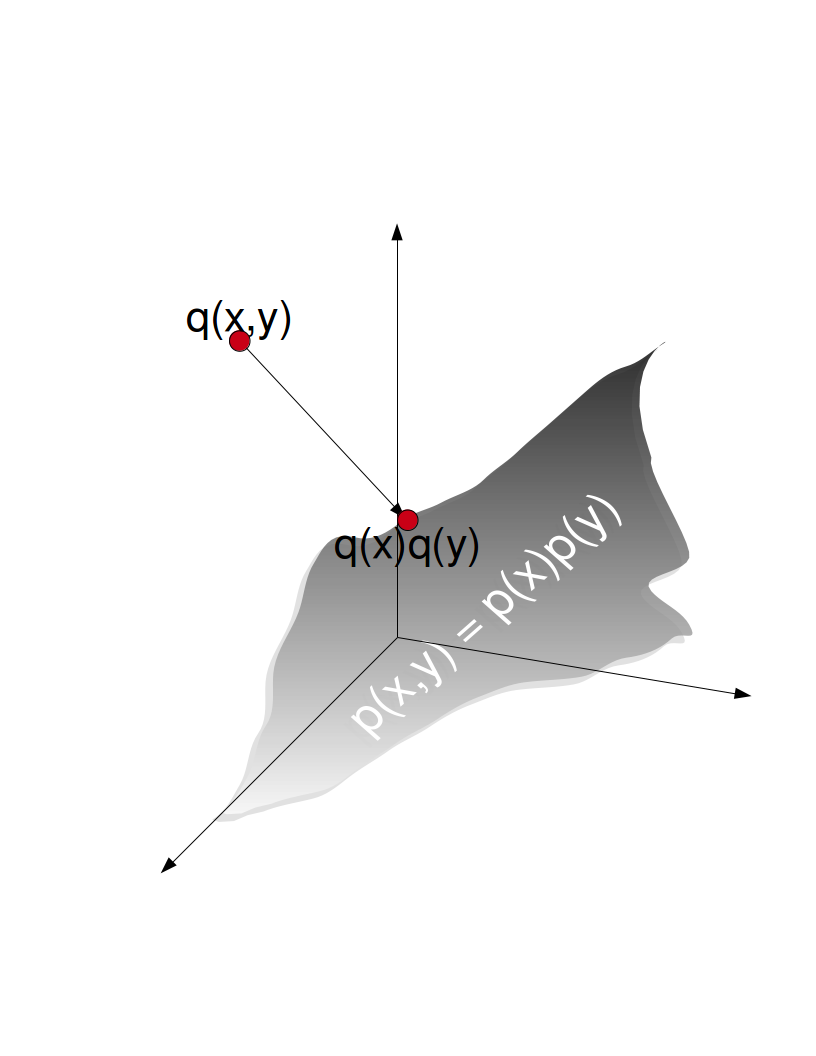
\includegraphics[width = \textwidth]{figuras/distributionmanyfold.png}
 	\caption[Representação pictórica da projeção de uma distribuição.]{ Representação pictórica da projeção de uma distribuição em uma certa família de distribuições convenientes. O espaço representado na figura corresponde de forma pictórica ao espaço formado por todas as distribuições de probabilidade. A superfície corresponde a um sub-espaço, nesse caso, o sub-espaço de distribuições fatoráveis, correspondentes a variáveis independentes. A projeção de uma distribuição qualquer $q(x,y)$ sobre esse sub-espaço através da minimização da divergência de Kullback-Leibler resulta na distribuição dada pelo produto das distribuições marginais $q(x)q(y)$. }
       \label{fig:distributionmanyfold}
\end{figure}
\begin{equation}
\label{eq:infomutua}
I(X_1,\ldots, X_n) = \min_{\{\phi_i(x_i)\}} \int p(x_1,\ldots, x_n) \log \frac{p(x_1,\ldots, x_n)}{\prod_{i=1}^{n}\phi_i(x_i)} \prod_{i=1}^{n}\ud x_i
\end{equation}
Fazendo a derivada funcional da expressão a ser minimizada com relação às distribuições indeterminadas $\phi_k(x)$ obtemos a condição de extremo, com o vínculo de que as distribuições $\phi_j(x)$ sejam normalizadas:
\begin{equation}
 \phi_k(x_k) = \int  p(x_1, x_2, \ldots, x_n) \prod_{i\ne k}\ud x_i = p_{X_k}(x_k)
\end{equation}
Ou seja: a distribuição $\phi_j(x_j)$ devem ser a distribuição marginal da variável $X_j$, e podemos reescrever:
\begin{equation}
\label{eq:infomutua2}
 I(X_1,\ldots, X_n) = \int p(x_1,\ldots, x_n) \log \frac{p(x_1,\ldots, x_n)}{\prod_{i=1}^{n} p_{X_i}(x_i)} \prod_{i=1}^{n}\ud x_i
\end{equation}
Esse funcional que mede a dependência mútua entre grupos de variáveis é denominado Informação Mútua ou Correlação Total\footnote{Alguns autores reservam o nome Informação Mútua para o caso de duas variáveis}. Interpretações para a o funcional podem ser obtidas notando que:
\begin{align}
 I(X_1,\ldots, X_n) &= \sum_{i=1}^{n} H(X_i) - H(X_1, \ldots, X_n)  \label{eq:entropydecomposition}\\
		    &= H(X_j) - H(X_j | X_1, \ldots, X_{j-1}, X_{j+1}, \ldots, X_n) 
\end{align}
Dessa forma, pode-se interpretar $I(X_1, \ldots, X_n)$ como a redução na incerteza a respeito da variável $X_j$ proporcionada pelo conhecimento das variáveis $X_1, \ldots, X_{j-1}, X_{j+1}, \ldots, X_n$. A informação mútua para duas variáveis, dada por:
\begin{equation}
\label{eq:infomutuabiv}
 I(X,Y) = \int \ud x\,\ud y\; p(x, y) \log \frac{p(x, y)}{p_{X}(x),p_{Y}(y))},
\end{equation}
satisfaz todos os critérios discutidos na seção anterior para ser uma boa medida de dependência. 
\section{Cópulas}
\newthought{A elucidação do conceito de dependência} eventualmente se choca com a noção de cópula\cite{Nelsen2006}. Um teorema devido a Sklar\cite{Sklar1959} permite separar a distribuição cumulativa conjunta - $F_{X,Y}(x,y)$ - de duas variáveis em duas partes: (a) as distribuições cumulativas marginais de cada variável - $F_{X}(x)$ e $F_{Y}(y)$, que trazem informação idiossincrática a respeito de cada uma das variáveis (b) e uma função cópula C(u,v), que traz informação sobre a dependência entre as variáves. De maneira geral o teorema de Sklar pode ser enunciado da seguinte forma:
\begin{Teorema}[Teorema de Sklar]
Para toda distribuição cumulativa conjunta contínua de duas variáveis $F_{XY}(x,y)$, com distribuições cumulativas $F_X(x)$ e $F_Y(y)$, existe uma função cópula única $C(u,v)$ tal que:
\begin{equation}
 F_{XY}(x,y) = C(F_{X}(x), F_{Y}(y)).
\end{equation}
Similarmente, dadas quaisquer duas distribuições cumulativas univariadas $F_X(x)$ e $F_Y(y)$ e uma função cópula $C(u,v)$, é possível construir uma distribuição conjunta dada por $F_{XY}(x,y) = C(F_X(x),F_Y(y))$.
\end{Teorema}

\newthought{A própria função cópula} é uma legítima distribuição cumulativa conjunta, associada às variáveis $U = F_{X}(X)$ e $V = F_{Y}(Y)$:
\begin{equation*}
 F_{UV}(u,v) = C(u,v)
\end{equation*}
Dessa forma, podemos também definir a densidade de cópula, a densidade de probabilidade das variávies $U$ e $V$:
\begin{equation*}
 p_{UV}(u,v) = c(u,v) = \frac{\partial^2 C}{\partial u \partial v}
\end{equation*}
Essa definição implica que a densidade de probabilidade conjunta das variáveis $X$ e $Y$ é dada por:
\begin{equation}
\label{eq:density}
 p_{XY}(x,y) = c(F_X(x), F_Y(y)) p_X(x) p_Y(y)
\end{equation}
Dessa forma, o teorema de Sklar permite dividir a informação contida na distribuição conjunta em duas partes: 
\begin{itemize}
 \item uma parte que diz respeito apenas às propriedades de cada uma das variáveis -- que é dada pelas distribuições marginais;
 \item e uma parte que diz respeito à dependência estatística entre as duas variáveis -- que é dada pela função cópula. 
\end{itemize}
 
\subsection{Exemplos}
\label{sec:exemplos}
\newthought{Como exemplos de funções cópula} temos as cópulas associadas às distribuições multivariadas mais comumente utilizadas. Qualquer família de distribuições multivariadas  com um conjunto de parâmetros $\theta$ dada por $p(x,y |\theta)$ define uma função cópula dada por:
\begin{equation}
\label{eq:generalcopula}
C(u,v|\theta) = \int_{-\infty}^{F_{X}^{-1}(u)} \int_{-\infty}^{F_{X}^{-1}(v)} \ud x \ud y p(x,y|\theta)
\end{equation}
A cópula mais comumente empregada em todo tipo de análise estatística é a cópula normal ou gaussiana que, argumentaremos mais adiante, postula a mínima dependência linear entre duas variáveis:
\begin{equation}
 \label{eq:normalcop}
 N_{\rho}(u,v) = \frac{1}{2\pi\sqrt{1 - \rho^2}}\int_{-\infty}^{\Phi^{-1}(u)} \int_{-\infty}^{\Phi^{-1}(v)} \ud u \ud v\; e^{-\frac{u^2 + v^2 - 2uv\rho}{2(1-\rho^2)}}
\end{equation}
onde $\Phi(x) = \frac{1}{\sqrt{2\pi}}\int_{-\infty}^{x} \exp{-u^2/2} \ud u$ é a distribuição cumulativa normal padronizada. A família de cópulas normais depende apenas de um parâmetro $\rho \in [-1,1]$ que, \textit{no caso em que sejam inseridas marginais gaussianas para formar uma distribuição conjunta}, é igual à correlação entre as variáveis assim distribuidas. É importante notar que, para quaisquer outras marginais, a correlação poderá uma função do parâmetro $\rho$ e de quaisquer outros parâmetros dessas distribuições marginais. Essa família contém a cópula de variáveis independentes $C(u,v) = uv$ quando $\rho = 0$.

\newthought{Uma cópula ligeiramente mais complicada que a normal} é a cópula associada à distribuição t de Student que, além da dependência linear descrita pelo parâmetro $\rho$, apresenta também dependência nas caudas da distribuição. A distribuição t de Student bivariada padrão\footnote{Médias não-nulas e variância diferente da unitária podem ser trivialmente acrescentadas através de translações e mudanças de escala. Uma vez que essas transformações só afetam as marginais e mantém a cópula invariate - são trasformações inversíveis, coordenada a coordenada - não afetam a dependência} é dada por:
\begin{equation}
\label{eq:tbivariada}
p_{T}(x,y\mid  \rho, \nu) = \frac{\Gamma(1+\frac{\nu}{2})}{\Gamma(\frac{\nu}{2}){\pi\nu\sqrt{1-\rho^2}}}\left[1+ \frac{q_\rho(x,y)}{\nu}\right]^{-(1+\frac{\nu}{2})},
\end{equation}
onde $q_\rho(x,y) = \frac{1}{1-\rho^2}\left[x^2+ y^2 - 2\rho xy\right]$. As marginais dessa distribuição são distribuições t univariadas:
\begin{equation}
\label{eq:tunivariada}
 p(x_i|\nu) = \frac{\Gamma(\frac{\nu+1}{2})} {\sqrt{\nu\pi}\,\Gamma(\frac{\nu}{2})} \left(1+\frac{x_i^2}{\nu} \right)^{-(\frac{\nu+1}{2})}\!
\end{equation}
No limite $\nu \to \infty$ essa distribuição se reduz à distribuição normal bivariada padronizada, com parâmetro de correlação linear $\rho$, médias nulas e variâncias unitárias. Para $\nu$ finito as marginais adquirem caudas pesadas e a dependência entre as variáveis ganham uma componente além da correlação linear - adicionando peso nas caudas da cópula. A cópula t pode ser obtida introduzindo essa distribuição na eq. \eqref{eq:generalcopula}:
\begin{equation}
 \label{eq:tcop}
C_{T}(u,v|\nu, \rho) = \frac{\Gamma(1+\frac{\nu}{2})}{\Gamma(\frac{\nu}{2}){\pi\nu\sqrt{1-\rho^2}}}
\int_{-\infty}^{t_\nu^{-1}(u)} \int_{-\infty}^{t_\nu^{-1}(u)} \ud x \ud y
{\left[1+ \frac{q_{\rho}(x,y)}{\nu}\right]^{-\frac{\nu+2}{2}}}
\end{equation}
onde $t_{\nu}(x)$ é a distribuição cumulativa associada à distribuição univariada em \eqref{eq:tunivariada}.

\newthought{Uma terceira família de cópulas} que convém citar são as cópulas arquimedianas, que podem ser escritas como:
\begin{equation}
\label{eq:arqcop}
C(u,v | \Psi(\cdot)) = \Psi^{-1}\left(\Psi(u) + \Psi(v)\right)
\end{equation}
parametrizadas por uma função $\phi$. Essas funções cópula existem desde que: $\Psi(1) = 0$, $\lim_{x \to 0}\Psi(x) = \infty$, $\Psi'(x) < 0$ e $\Psi''(x) > 0$. Essa família contém a cópula de variáveis independentes quando $\Psi(x) = -\log(x)$.
\subsection{Dependência extrema - limites de Frechet-Hoeffding}

\newthought{A definição de cópula} permite tornar mais preciso o conceito de dependência extrema. As equações \eqref{eq:independence} e \eqref{eq:density} em conjunto nos permitem concluir que, para duas variáveis independentes:
\begin{align}
c(u,v) &= 1, \\
C(u,v) &= uv,
\end{align}
Para o caso de dependência completa é possível mostrar que\cite{Nelsen2006} toda cópula está limitada por duas funções que representam dependência máxima, denominadas limites de Frechet-Hoeffding. Essas funções são:
\begin{align}
\label{eq:frechethoeffding}
W(u,v) &= \max(0, u+v-1) \\
M(u,v) &= \min(u,v)
\end{align}
Essas duas funções são elas próprias cópulas e limitam por cima e por baixo todas as outras cópulas possíveis:
\begin{equation}
W\left(u,v\right) \le C(u,v) \le M(u,v)  
\end{equation}
para qualquer possível cópula $C(u,v)$. As densidades de cópula associadas a essas duas funções evidenciam que casos descrevem:
\begin{align}
w(u,v) &= \delta(u+v) \\
m(u,v) &= \delta(u-v).
\end{align}
Inserindo marginais F(x) e G(y) quaisquer, nota-se o tipo de distribuições conjuntas que essas cópulas geram: ambas descrevem duas variáveis com dependência monotônica - crescente no caso de $M$ e decrescente no caso de $W$.

\subsection{Medidas de dependência revisitadas}

\newthought{Os ``axiomas'' de Rényi} a respeito de medidas de dependência podem ser revisitados e tornados mais precisos com o conceito de cópula e cópulas extremas em mãos. Os itens \ref{item:funcional}, \ref{item:simétrico} e \ref{item:invariante} ficam imediatamente satisfeitos se a medida de dependência em questão for funcional apenas da cópula e não das distribuições marginais. Além disso, os itens \ref{item:indep} e \ref{item:maximo} podem ser reescritos em termos das cópulas extremas e da cópula independente. Podemos reescrever então esses requisitos da seguinte forma:
\begin{itemize}
\item Uma boa medida de dependência entre duas variáveis $X$ e $Y$ é um funcional $\mathcal{F} : C_{2} \to \mathcal{R}$ que leva funções cópula $C_{XY}(\cdot, \cdot)$ em números reais e independe das distribuições marginais;
\item atinge um valor mínimo, que será arbitráriamente escolhido como zero, se, e somente se, $C_{XY}(u,v) = uv$;
\item atinge um valor máximo quando $C_{XY}(u,v) = W(u,v)$ ou $C_{XY}(u,v) = M(u,v)$.
\item para $C_{XY}(u,v) = N_{\rho}(u,v)$, o funcional é um função monotônica crescente do parâmetro  $\rho$. 
\end{itemize}
A correlação linear falha em dois itens: é possível representar a correlação linear como função da cópula, mas não é possível eliminar sua dependência com as marginais:
\begin{equation*}
 \hat{\rho}_{X,Y} = \frac{1}{\sigma_X\sigma_Y}\int\int C(u,v) \ud F_{X}^{-1}(u) \ud F_{X}^{-1}(v).
\end{equation*}
Essa expressão depende das marginais explicitamente nas medidas de integração e implicitamente nas variâncias $\sigma_i$. Além disso, a correlação não atinge seus valor extremo sempre que a cópula escolhida como uma das cópulas de Frechet-Hoeffding - o valor assumido nesse caso depende das marginais específicas. Outras medidas apresentadas acima, o tau de Kendall ($\tau$) e a correlação de postos de Spearman ($\rho^{S}$) podem ser facilmente escritas de forma a satisfazer todas os critérios acima:
\begin{align}
\tau & = 4 \int_0^1\int_0^1 C(u,v) dC(u,v)  - 1  \\
\rho^{S} &=  12 \int_0^1\int_0^1 \left[C(u,v) - uv\right] du dv
\end{align}
O último requisito pode ser verificado notando-se que, para o caso de cópulas normais, essas expressões se reduzem a\footnote{A expressão para o tau de Kendall vale para toda distribuição elíptica, incluindo a distribuição t de Student}:
\begin{align}
\tau &= \frac{2}{\pi} \arcsin(\rho), \\
\rho^{S} &= \frac{6}{\pi} \arcsin\left(\frac{\rho}{2}\right).
\end{align}
Além disso, a Informação Mútua, como mostraremos na próxima seção, também satisfaz os requisitos acima.
\section{Entropia de Cópula}
\label{sec:copentropy}
\newthought{Para escrever} a informação mútua como um funcional da cópula basta recorrer à definição da densidade de cópula e a expressão da distribuição conjunta 
em termos desta, na eq. \eqref{eq:density} que reproduzimos abaixo:
\begin{equation*}
p_{XY}(x,y) = c(F_X(x), F_Y(y)) p_X(x) p_Y(y).
\end{equation*}
Usando essa expressão na definição de informação mútua eq. \eqref{eq:infomutuabiv}:
\begin{equation*}
 I(X,Y) = \int \ud x\,\ud y\; p(x, y) \log \frac{p(x, y)}{p_{X}(x),p_{Y}(y))},
\end{equation*}
temos:
\begin{align*}
 I(X,Y) &= \int p_X(x) \ud x\, p_Y(y)\ud y\; c(F_X(x), F_Y(y)) \log \left[c(F_X(x), F_Y(y)\right] \\&= \int \ud u \ud v\; c(u,v) \log c(u,v)
\end{align*}
e portanto:
\begin{equation}
\label{eq:copulaentropy}
I(X,Y) = \int \int \ud u \ud v \; c(u,v) \log c(u,v)  = - S[c] \ge 0
\end{equation}
onde $S[c]$ é a entropia associada à distribuição conjunta $c(u,v)$, daqui por diante denominada \textit{entropia de cópula} \cite{Ma2008,Jenison2004}.
Esse resultado oferece ainda mais uma interpretação aos múltiplos significados da informação mútua - que ressoa diretamente com a definição de dependência apresentada no início deste capítulo - é o conteúdo de informação associado à dependência entre duas variáveis. A combinação desse resultado com a eq. \eqref{eq:entropydecomposition} permite escrever\footnote{A expressão acima pode ser imediatamente generalizada para um número arbitrário de variáveis}:
\begin{equation}
\label{eq:entropydecomposition2}
H(X_1, X_2, \ldots, X_N) = \sum_{i=1}^{N} H(X_i) + H_{\mbox{cop}} 
\end{equation}
decompondo então a entropia, o conteúdo informacional da distribuição conjunta, em parcelas devidas às características de cada uma das variáveis e uma parcela correspondente ao acoplamento entre essas variáveis. Eq. \eqref{eq:copulaentropy} também oferece um conveniente princípio para encontrar cópulas informacionalmente neutras segundo o princípio de máxima entropia\cite{Jaynes2003}: a cópula menos informativa é a que postula a menor informação mútua possível entre as variáveis. 

\newthought{O último passo} para mostrar que a informação mútua satisfaz todos os critérios para ser uma boa medida de dependência é notar que, no caso de cópulas gaussianas:
\begin{equation}
\label{eq:infonormal}
I(X_1,X_2) =  - \frac{1}{2}\log\left(1 - \rho^2\right)
\end{equation}
\section{``Excesso'' de informação mútua}
\subsection{Correlação Linear \textit{vs.} parâmetro }
\newthought{A distribuição de máxima entropia} que satisfaz vínculos de que correlação, médias, e variâncias de um par de variáveis $X$ e $Y$ assumam certos valores é a distribuição normal. Usando a decomposição da eq. \eqref{eq:entropydecomposition2}, temos, uma vez que as entropias das marginais dependem apenas das variâncias e a informação mútua apenas da correlação\footnote{Note a importância de separar conceitualmente o parâmetro correlação, que identifica uma certa distribuição na família de distribuições normais, do funcional são homônimos, o qual estamos chamado de ``correlação linear'' e que está definido para qualquer distribuição.}:
\begin{equation*}
H(X_1,X_2) = h(\sigma_1) + h(\sigma_2) + \frac{1}{2}\log\left(1 - \hat{\rho}^2\right)
\end{equation*}
onde $h(\sigma)$ é a entropia de uma distribuição normal univariada com variância $\sigma^2$. Se essa é a maior possível entropia dada a correlação e variâncias, e uma vez que a informação mútua independe das variâncias\footnote{Pois independe das marginais.}, então o valor:
\begin{equation}
\label{eq:mutinfogaussian}
 I_{0}(\hat{\rho}) = - \frac{1}{2}\log\left(1 - \hat{\rho}^2\right)
\end{equation}
é um limite inferior para a informação mútua de qualquer par de variáveis que tenham correlação $\hat{\rho}$:
\begin{equation}
\label{eq:gaussianinequality}
 I_{XY} \ge I_{0}(\hat{\rho}_{XY}).
\end{equation}
Dessa forma, representando formalmente em um plano $I\;\mbox{\textit{vs}.}\;\hat{\rho}$ as possíveis distribuições conjuntas com cópula gaussiana\footnote{Essa representação não é única. Está sendo empregada apenas como ilustração. Essas duas grandezas não formam um bom sistema de coordenadas para a variedade de distribuições com cópula gaussiana.}, temos a figura \ref{fig:correlinfomutua}.
\begin{figure}
 \centering
 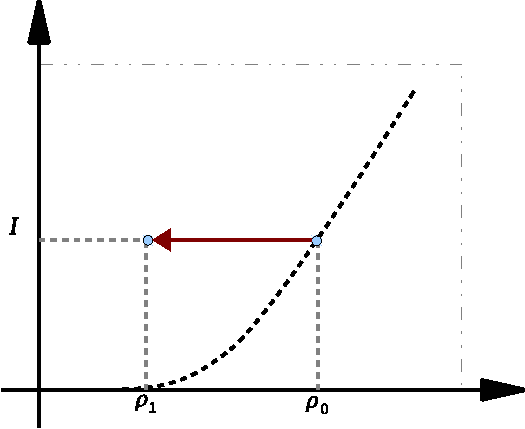
\includegraphics[width = 0.6\textwidth]{./figuras/fig1-mod.pdf} 
 \caption[ A correlação linear é subestimada no caso de marginais não-Gaussianas.]{A correlação linear é subestimada no caso de marginais não-Gaussianas. Se ambas as marginais são Gaussianas, a distribuição conjunta está localizada sobre o limite inferior para a informação mútua. Uma mudança nas marginais mantendo fixa a cópula, preserva a informação mútua, entretanto a correlação estimada deve se deslocar para valores de menor módulo.}
 \label{fig:correlinfomutua}
\end{figure}

\newthought{Nessa figura} temos duas distribuições destacadas. Uma delas possui marginais gaussianas, sendo portanto uma distribuição normal bivariada e deve estar localizada sobre a curva $I_{0}(\hat{\rho})$, representada pela linha escura tracejada. Para essa distribuição o parâmetro $\rho$, uma boa medida de dependência se restrito a cópulas gaussianas, é exatamente igual à correlação linear $\hat{\rho}$. Se as marginais forem trocadas por marginais não-gaussianas, a informação mútua, independente das marginais, deve permanecer a mesma. Entretanto a correlação, como argumentado acima, deve mudar com a troca de marginais. Uma vez que uma mudança para valores maiores do módulo da correlação linear violaria a condição $I\ge I_{0}(\hat{\rho})$, a única alternativa é que o módulo da correlação diminua. Dessa forma, teríamos uma distribuição conjunta que tem cópula gaussiana com parâmetro $\rho_0$ e correlação linear $\hat{\rho} < \rho_{0}$. Uma tentativa de identificar o parâmetro $\rho$ da cópula gaussiana com a correlação linear levaria a atribuir ao par de variáveis uma dependência menor - talvez muito menor - do que a real. Em muitas aplicações isso pode ser perigoso. Em particular em aplicações financeiras o risco de uma operação pode ser subestimado por se subestimar a frequencia de co-ocorrência de eventos negativos. É notório que séries temporais financeiras apresentam distribuições marginais com caudas pesadas - e portanto distantes de uma gaussiana. O uso, bastante difundido\cite{FT2009}, de cópulas gaussianas para estimativa de risco combinado com o uso de estimadores baseados na correlação linear nessas condições pode significar que o risco de uma posição é substancialmente maior do que o estimado. Um dos requisitos para uma boa medida de dependência é que, para o caso de cópulas gaussianas, a medida em questão seja função monotônica e crescente do módulo do parâmetro $\rho$. Dessa forma, qualquer outra medida de dependência é mais adequada que a correlação linear para estimar a dependência de fato entre duas variáveis com dependência gaussiana.

\subsection{Informação mútua para cópulas elípticas}

\newthought{O tau de Kendall} é um estimador ainda mais completo para $\rho$: ele é uma função monotônica do parâmetro $\rho$ para qualquer cópula pertencente à família elíptica - da qual a gaussiana é um caso particular. Uma distribuição é dita elíptica sempre que: 
\begin{equation}
\label{eq:eliptical}
\avg{e^{i\vec{k}\cdot\vec{x}} } = e^{i\vec{\mu}^{T}\vec{k}} \psi\left(i\frac{\vec{k}^{T}\Sigma\vec{k}}{2}\right),
\end{equation}
onde $\Sigma$ é a matriz de covariância e $\vec{\mu}$ o vetor de valores esperados de $\vec{x}$. Uma distribuição elíptica padronizada é aquela em que as médias são nulas e todas as variâncias unitárias, de modo que a matriz de covariâncias é igual à matriz de correlações - $\Sigma_{ij} = \rho_{ij}$. Denotaremos essa família de distribuições por $p(\vec{x} | \Sigma, \psi(\cdot))$. No caso de $\Sigma_{ij} = \delta_{ij}$, a distribuição é invariante por rotações no vetor $\vec{x}$ e é dita uma \textit{distribuição esférica} - na família 
$p(\vec{x} | \psi(\cdot))$. 

\newthought{É possível ver uma variável distribuida} com respeito a uma distribuição elíptica $\vec{x} \sim p(\vec{x} | \Sigma, \psi(\cdot))$ como uma transformação linear de variáveis distribuidas com relação à distribuição esférica com o mesma função $\psi(\cdot)$: 
\[
x_{i} = \sum_{j} A_{ij} y_{j} 
\]
Onde $\Sigma = A^{T}A$ e $\vec{y}\sim p(\vec{y}| \psi(\cdot))$. Cópulas elípticas são as cópulas associadas a essas distribuições e têm como parâmetros as correlações de pares - $\rho_{ij}$ - e a função $\psi(\cdot)$. A eq.\eqref{eq:eliptical} é uma transformação de Fourier, que sempre pode ser invertida para obter a distribuição conjunta. No caso de distribuições elípticas padrão, temos:
\[
p(\vec{x}| \Sigma, \psi(\cdot) )  = \int \frac{\ud^N k}{(2\pi)^N} e^{-i\vec{k}^{T}\vec{x}} \psi\left(i\frac{\vec{k}^{T}\Sigma\vec{k}}{2}\right) 
\]
podemos introduzir uma função delta e obter:
\[
p(\vec{x}| \Sigma, \psi(\cdot) )  = \int \ud u \int \frac{\ud^N k}{(2\pi)^N} e^{-i\vec{k}^{T}\vec{x}} \psi\left(u\right) \delta\left(u - i\frac{\vec{k}^{T}\Sigma\vec{k}}{2}\right) 
\]
e usando a representação integral da função delta:
\begin{align*}
p(\vec{x}| \Sigma, \psi(\cdot) )  &= \int \frac{\ud u \ud \hat{u}}{2\pi} \int \frac{\ud^N k}{(2\pi)^N}  \psi\left(u\right) \exp\left[i\hat{u}\left(u - i\frac{\vec{k}^{T}\Sigma\vec{k}}{2}\right)-i\vec{k}^{T}\vec{x}\right] \\
		     &= \int \frac{\ud u \ud \hat{u}}{2\pi} e^{i\hat{u}u}\psi\left(u\right) \int \frac{\ud^N k}{(2\pi)^N}   \exp\left[\hat{u}\frac{\vec{k}^{T}\Sigma\vec{k}}{2}-i\vec{k}^{T}\vec{x}\right]
\end{align*}
A integral gaussiana sobre $\vec{k}$ pode ser feita e temos:
\begin{align*}
p(\vec{x}| \Sigma , \psi(\cdot))  &= \int \frac{\ud u \ud \hat{u}}{2\pi} e^{i\hat{u}u}\psi\left(u\right) N(x | \hat{u} \Sigma) \\
		     &= \int \ud u \; p(u) N(x | u \Sigma)  = 
\end{align*}
onde $N(x|\Sigma)$ é a distribuição normal padronizada com matriz de correlação $\Sigma$ e $p(u) = \int \ud u e^{ivu}\psi(v)$ é uma certa função ligada à transformada de Fourier de $\psi(u)$. Essa representação para as distribuições elípticas pode ser entendida da seguinte forma: $p(\vec{x} | \Sigma, \psi(\cdot))$ é a distribuição resultante quando se toma $\vec{x}$ de uma gaussiana de matriz de correlação $u\Sigma$ em que $u$ é sorteado de acordo com uma distribuição $p(u)$. Dessa forma podemos, de forma alternativa, parametrizar a família elíptica pela distribuição $p(u)$ - $p(\vec{x} | \Sigma, p(\cdot))$. Também podemos escrever de forma mais explícita:
\begin{align}
 p(\vec{x} | \Sigma , p(\cdot)) &= \frac{1}{\sqrt{(2\pi)^N |\Sigma|}} \int \ud^N u\;\frac{1}{u^{N/2}} p(u) e^{-\frac{1}{2u} \vec{x}^{T} \Sigma^{-1} \vec{x}}  \\
		     &= \frac{1}{\sqrt{(2\pi)^N |\Sigma|}} \Psi_{N}\left(-\frac{1}{2} \vec{x}^{T}\Sigma^{-1}\vec{x}\right) \label{eq:elipjoint}
\end{align}
onde definimos: $\Psi_j(q) = \int \ud^j u \; \frac{1}{u^{j/2}} p(u) e^{-\frac{q}{u}}$. As marginais de uma distribuição elíptica podem ser facilmente calculadas notando-se que as marginais da normal padronizada são distribuições normais padronizadas sobre 1 variavel. Dessa forma:
\begin{equation}
\label{eq:elipmarginal}
 p_j(x_j) = \frac{1}{\sqrt{2\pi}}\int \ud u \;\frac{1}{\sqrt{u}} p(u) e^{-\frac{x_j^2}{2u}} = \frac{1}{\sqrt{2\pi}} \Psi_{1}\left(\frac{x_j^2}{2}\right)
\end{equation}
Finalmente de posse dessas das eqs. \eqref{eq:elipjoint} e \eqref{eq:elipmarginal} podemos mostrar a seguinte proposição.
\begin{Proposicao}[Decomposição da informação mútua de uma cópula elíptica]
Se $C(u,v | \Sigma, p(\cdot))$ é uma cópula elíptica com matriz de correlação $\Sigma$, então a informação mútua associada pode ser decomposta na forma:
\begin{equation}
  I(\Sigma, \psi(\cdot)) = I_{0}(\Sigma) + I[p(\cdot)],
\end{equation}
onde $I_{0}(\Sigma) = -\frac{1}{2}\log\Sigma$ é a informação mútua de uma cópula gaussiana com matriz de correlação $\Sigma$ e $I[p(\cdot)]$ é um funcional de $p(u)$ que é igual à informação mútua da distribuição esférica correspondente e independe da matriz de correlação. 
\end{Proposicao}
\begin{proof}
Para mostrar essa proposição recorremos à eq.\eqref{eq:entropydecomposition}:
\begin{equation*}
I = \sum_{i}^{N}H[X_j] - H[\vec{x}] = N H[X_1] - H[\vec{x}]
\end{equation*}
onde a segunda igualdade é obtida notando que as marginais $p_j(\cdot)$ são todas idênticas. A primeira parcela já é um funcional de p(u) que independe da matriz de correlação que pode ser escrito como: 
\begin{align*}
N H[X_1] &= N\int \ud x \frac{1}{\sqrt{2\pi}} \Psi_{1}\left(\frac{x^2}{2}\right) \log\left[\frac{1}{\sqrt{2\pi}} \Psi_{1}\left(\frac{x^2}{2}\right)\right] \\
	 &= \int \ud^N x \frac{1}{\sqrt{(2\pi)^N}} \Psi_{N}\left(-\frac{1}{2} \vec{x}^{T}\vec{x}\right) \log\left[\frac{1}{\sqrt{(2\pi)^N}}\prod_j \Psi_{1}\left(\frac{x_j^2}{2}\right)\right]
\end{align*}
A segunda parcela pode ser explicitamente escrita como:
\begin{equation*}
 H[\vec{x}] = - \int \ud^N x \frac{1}{\sqrt{(2\pi)^N |\Sigma|}} \Psi_{N}\left(-\frac{1}{2} \vec{x}^{T}\Sigma^{-1}\vec{x}\right) \log\left[\frac{1}{\sqrt{(2\pi)^N |\Sigma|}} \Psi_{N}\left(-\frac{1}{2} \vec{x}^{T}\Sigma^{-1}\vec{x}\right)\right]
\end{equation*}
A inversa da matriz de correlação é simétrica e quadrada, e portanto sempre pode ser escrita como $\Sigma^{-1} = U^{T} \Lambda U$, onde U é uma matriz unitária e $\Lambda_{ij} = \delta_{ij}\lambda_j$ é uma matriz diagonal dos autovalores de $\Sigma^{-1}$. Fazendo a mudança de variáveis $\vec{y} = U\vec{x}$ temos:
\[
H[\vec{x}] = - \int \ud^N y \frac{1}{\sqrt{(2\pi)^N |\Sigma|}} \Psi_{N}\left(-\frac{1}{2} \vec{y}^{T}\Lambda\vec{y}\right) \log\left[\frac{1}{\sqrt{(2\pi)^N |\Sigma|}} \Psi_{N}\left(-\frac{1}{2} \vec{y}^{T}\Lambda\vec{y}\right)\right]
\]
A matriz diagonal $\Lambda$ pode ser escrita como $\Lambda = D^{T} D$, onde $D_{ij} = \delta_{ij}\sqrt{\lambda_j}$. Fazendo a mudança de variáveis\footnote{Vamos renomear a nova variável de integração como $\vec{x}$ novamente por conveniência} $\vec{x}= D\vec{y}$, temos:
\begin{equation*}
 H[\vec{x}] = - \int \ud^N x \frac{1}{\sqrt{(2\pi)^N}} \Psi_{N}\left(-\frac{1}{2} \vec{x}^{T}\vec{x}\right) \log\left[\frac{1}{\sqrt{(2\pi)^N |\Sigma|}} \Psi_{N}\left(-\frac{1}{2} \vec{x}^{T}\vec{x}\right)\right]
\end{equation*}
Uma vez que $|D| = \prod_{i} \sqrt{\lambda_i} = \frac{1}{\sqrt{|\Sigma|}}$. O termo que contém $|\Sigma|$ dentro do logaritmo pode ser removido da integral\footnote[][-2cm]{Note que a normalização de p($\vec{x}$) exige que $\int \ud^N x \psi_{N}(\vec{x}^{T}\vec{x}) = \sqrt{(2\pi)^N}$} e ficamos com:
\begin{fullwidth}
\[
H[\vec{x}] = - \int \ud^N x \frac{1}{\sqrt{(2\pi)^N}} \Psi_{N}\left(-\frac{1}{2} \vec{x}^{T}\vec{x}\right) \log\left[\frac{1}{\sqrt{(2\pi)^N}} \Psi_{N}\left(-\frac{1}{2} \vec{x}^{T}\vec{x}\right)\right] + \frac{1}{2}\log|\Sigma|
\]
\end{fullwidth}
\newpage
e finalmente podemos escrever\footnote{No caso bivariado essa expressão se reduz à expressão \ref{eq:mutinfogaussian}}:
\begin{equation}
I = I[p(u)] - \frac{1}{2}\log|\Sigma|
\end{equation}
onde:
\begin{equation}
\label{eq:excesselliptical}
I[p(u)] = \int \ud^N x \frac{1}{\sqrt{(2\pi)^N}} \Psi_{N}\left(-\frac{1}{2} \vec{x}^{T}\vec{x}\right) \log\left[\frac{\Psi_{N}\left(-\frac{1}{2} \vec{x}^{T}\vec{x}\right)}{\prod_j \Psi_{1}\left(\frac{x_j^2}{2}\right)}\right]
\end{equation}
\end{proof}

\newthought{Essa proposição} nos permite escrever a informação mútua em duas parcelas - uma dependente da estrutura linear de dependência, relacionada à matriz de correlações, e uma parcela que contém informações sobre dependências não-lineares entre as variáveis. Uma vez que a informação mútua é sempre positiva, esse resultado nos permite ainda escrever uma versão mais forte da desigualdade eq.\eqref{eq:gaussianinequality} para o caso de cópulas elípticas:
\begin{equation}
\label{eq:gaussianineqgen}
 I_{XY} \ge I_{0}(\Sigma_{XY})
\end{equation}
onde, nesse caso, $\Sigma$ não é apenas a matriz de correlações lineares, mas o conjunto de parâmetros que identifica unicamente uma certa distribuição dentro de uma sub-família de cópulas elípticas com mesma função $\psi(\cdot)$.

\subsection{Excesso de Informação Mútua}

\newthought{As inequações eq.\eqref{eq:gaussianinequality} e eq.\eqref{eq:gaussianineqgen}} permitem concluir que a cópula gaussiana é a cópula de menor entropia dado o vínculo de dependências lineares representados por $\hat{\rho}$ ou $\Sigma$. Em outras palavras, a cópula gaussiana é a cópula que assume que uma variável tem a menor quantidade possível de informação a respeito de outra que ainda explica a parte linear da dependência. Além disso, a cópula gaussiana possui apenas a parte linear da informação mútua, e portanto representa uma dependência apenas linear entre as variáveis. O uso dessa cópula portanto representa uma hipótese implícita de dependência linear e mínima entre as variáveis. Caso essa hipótese falhe, um termo adicional deve surgir na informação mútua, que diz respeito à dependência não-linear. Esse termo será chamado ``excesso'' de informação mútua - entenda-se excesso com relação à cópula linear. A observação de um excesso de informação mútua permite criar um diagnóstico de ``gaussianidade'' da dependência entre duas variáveis. Para tal é necessário ser capaz de estimar o parâmetro $\rho$ da distribuição e a informação mútua. Para estimar $\rho$, empregaremos o tau de Kendall - uma medida que independe das marginais e permite estimar:
\begin{equation}
 \rho = \sin\left(\frac{\pi\tau}{2}\right).
\end{equation}
O tau de Kendall pode ser estimado empiricamente com um algoritmo simples: dado um conjunto de pontos $\{\vec{x}_\mu \sim p(\vec{x}) | \mu = 1,2,\ldots,P\}$, temos:
\begin{equation}
\label{eq:kendall}
\tilde{\tau}[X_i,X_j] = \binom{N}{2}^{-1} \sum_{\mu < \nu} \sign(x_\mu^i - x_\nu^i)\sign(x_\mu^j - x_\nu^j)
\end{equation}
onde a soma é feita sobre todos os pares $(\mu,\nu)$. Um método para estimação da informação mútua foi recentemente publicado por \citet{Kraskov2004}, baseado em estatísticas de k-vizinhos. Medindo $I$ e $\tau$ é possível diagnosticar um eventual ``excesso'' de informação mútua que, caso presente, indica que a dependência não é mínima e tem uma componente não-linear. Nesses casos a correlação linear não pode ser usada como medida de dependência. 
\begin{figure}
\subfloat[Todos os pares de ações.]{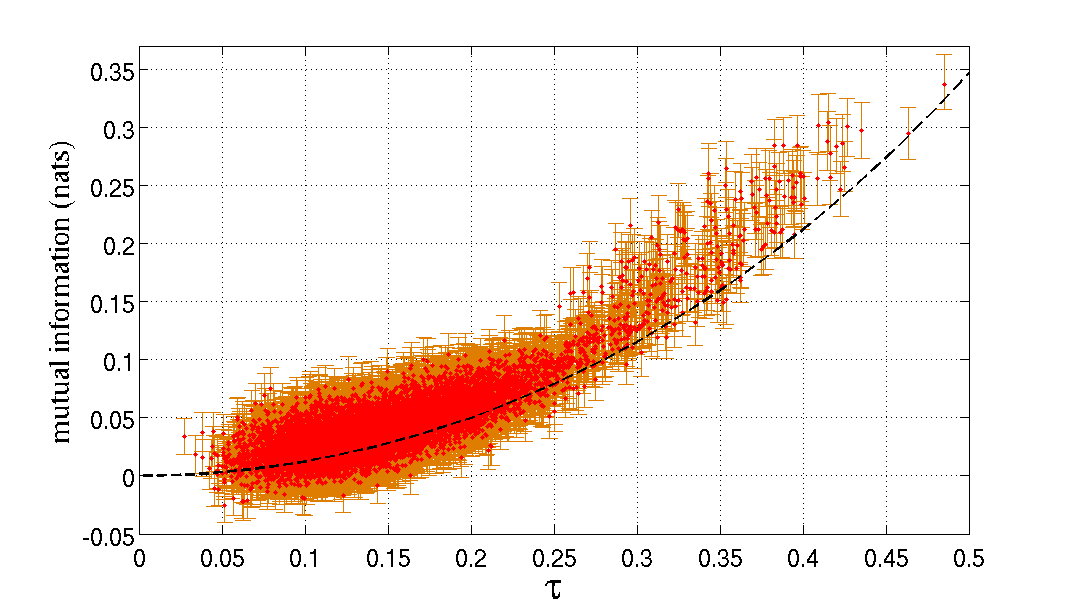
\includegraphics[width = \textwidth]{./figuras/MIvsrho_tau_final.png}}\\	
\subfloat[Seleção dos pares cujo limite inferior da barra de erro é maior que a informação mútua gaussiana - excesso de informação não nulo com $90\%$ de confiança (as barras de erro foram removidas para melhor visualização).]{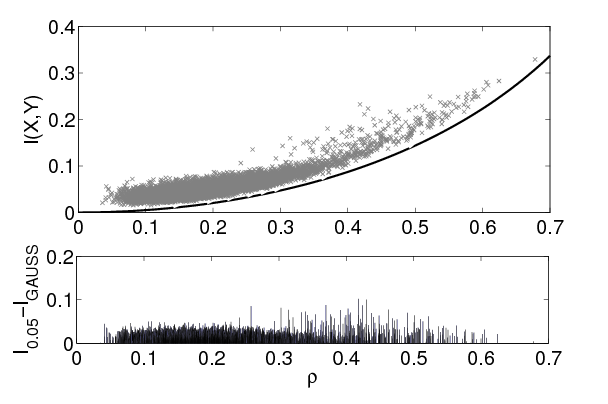
\includegraphics[width = \textwidth]{./figuras/IM_Pearson.png}}
\caption[Estimativas para a informação mútua \textit{vs.} tau de Kendall para séries financeiras.]{Estimativas para a informação mútua usando o algoritmo KSG contra o tau de Kendall (ou correlação medida via tau de Kendall) para pares de séries temporais de log-retornos diários $\log\frac{P_\text{close}}{P_\text{open}}$ (onde $P_\text{close}$ e $P_\text{open}$ são, respectivamente, preços dos ativos na abertura e fechamento diários do mercado) para 150 das ações mais negociadas que compõe o índice $S\&P500$, no período de 02/01/1990 a 16/09/2008 (aproximadamente 4700 pontos por série). As barras de erro representam intervalos de confiança de $90\%$ determinados segundo o procedimento de Bootstrap. Note que, nesse intervalo de confiança, um grande número de pares apresentam um excesso de informação mútua não-nulo com respeito à cópula gaussiana. As linhas tracejadas indicam o limite gaussiano para a informação mútua.}
\label{fig:acoes}
\end{figure}
Como exemplo desse diagnóstico, mostramos na figura \ref{fig:acoes} estimativas para essas quantidades para séries temporais de uma seleção de 150 das 500 ações que compõe o índice S\&P500, um índice de ações de alta capitalização negociadas em bolsas da NYSE Euronext e da NASDAQ OMX definido e mantido pela Standard \& Poor's. As barras de erro para a informação mútua, que representam um intervalo de confiança de $90\%$, foram calculadas usando o método de bootstrap, repetindo a estimativa do algoritmo KSG\cite{Kraskov2004} para diversas amostragens com repetição dos dados.
\begin{figure}
 \subfloat[Seleção de pares com baixa correlação e grande excesso de informação mútua]{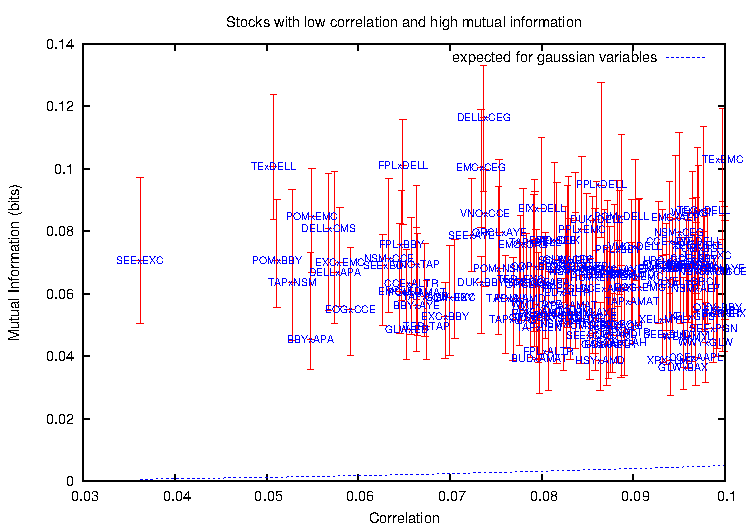
\includegraphics[width =\textwidth]{./figuras/locohimi.pdf}}\\
 \subfloat[Seleção dos pares compatíveis com uma distribuição gaussiana com $90\%$ de confiança.]{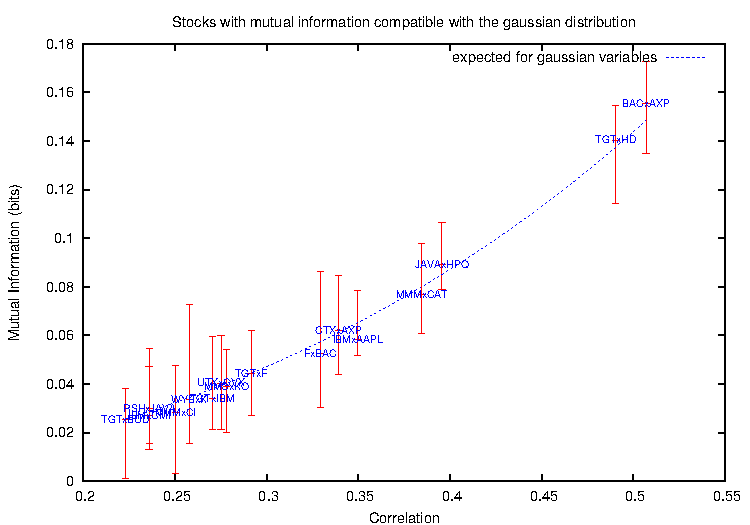
\includegraphics[width = \textwidth]{./figuras/gausscompat.pdf}}
 \caption[Seleção de pares de ações.]{Seleção de pares de ações com baixa correlação e grande excesso de informação mútua e pares compatíveis com uma distribuição gaussiana. Modelos modelos de risco baseados em medidas de correlação linear devem ser adequados para o segundo grupo e devem falhar seriamente para o primeiro.}
 \label{fig:locohimi}
\end{figure}
 O tau de Kendall foi também estimado usando procedimentos padrão como o da eq.\eqref{eq:kendall}. Observa-se que uma boa quantidade de pontos apresentam, dentro do intervalo de confiança, um valor para informação mútua não compatível com uma cópula gaussiana. Isso sugere que técnicas de avaliação e administração de risco baseadas no uso de cópulas gaussianas podem subestimar de forma substancial a dependência entre duas ações e o grau de co-movimento que elas apresentam. Na figura \ref{fig:locohimi} por exemplo, mostramos alguns pares de ações com correlações muito pequenas ($\rho < 0.1$) e que no entanto apresentam informação mútua compativel dependência muito maior do que a capturada por essa medida linear. 

\subsection{Ajuste empírico de cópulas via informação mútua}
\label{sec:ajuste}
\newthought{A determinação de uma particular cópula} para realizar essas medidas de risco poderia ser uma alternativa ao uso cego da cópula gaussiana. Uma possível forma de realizar essa determinação é minimizar a divergência de Kullback-Leibler entre a cópula empírica e uma família $\mathcal{C}_\theta$ de cópulas parametrizadas por um conjunto de parâmetros $\theta$:
\begin{equation}
 D[C(\vec{u}) || C(\vec{u} | \theta)] = \int \ud^N u \; c(\vec{u}) \log \frac{c(\vec{u})}{c(\vec{u}|\theta)}
\end{equation}
A minimização desse funcional com respeito a $\theta$ fornece uma possível cópula $c(\vec{u}|\theta^{\star})$ que é a mais próxima possível da cópula real dentro dessa família. Essa expressão pode ser manipulada da seguinte forma:
\begin{align}
D[\cdot|\cdot] &= \int \ud^N u \; c(\vec{u}) \log c(\vec{u}) - \int \ud^N u \; c(\vec{u}) \log c(\vec{u} | \theta) \\
&= I - L_{\infty}(\theta) 
\end{align}
onde o primeiro termo é o negativo da entropia de cópula, igual à informação mútua, como mostrado anteriormente, e o segundo termo é o valor assintótico da log-verossimilhança quando o número de amostras é grande:
\[
 L_{N}(\theta) = \frac{1}{N} \sum_{\mu=1}{N} \log c(\vec{u}_{\mu} | \theta)
\]
Uma vez que $D[|]\ge 0$ e $I \ge 0$, então minimizar a divergência de Kullback-Leibler, cujo menor valor possível é nulo, é equivalente a maximizar a log-verossimilhança com a informação mútua como limite. Se a log-verossimilhança fosse conhecida analíticamente isso poderia ser feito de maneira imediata resolvendo a equação:
\[
 L_{\infty}(\theta) = I
\]
Para um $I$ determinado empiricamente a partir dos dados,numericamente se necessário. Não há garantia alguma, no entanto de que há solução. Apenas haverá solução para essa equação se a própria cópula original fizer parte da família $\mathcal{C}_\theta$. Nesse caso a solução é única. Além disso não é possível conhecer $L_\infty$ analiticamente sem conhecer a cópula e uma aproximação é necessária. Supondo que a família de cópulas $\mathcal{C}_\theta$ é suficientemente próxima da cópula original, podemos substituir $c(\vec(u))$ pela própria $c(\vec{u}|\theta)$ na integral e aproximar $L_\infty(\theta)$ pela informação mútua de $c(\vec{u}|\theta)$. Dessar forma ficamos com uma espécie de método de ``correspondência de momentos'' (moment matching): deve ser escolhida na família $\mathcal{C}_\theta$ a cópula que tem mesma informação mútua que a empiricamente obtida:
\[
 I(\theta) = I.
\]
Novamente, não há garantia de solução, e agora nem mesmo da unicidade da solução. Mas a cópula escolhida certamente será capaz de descrever uma estrutura de dependência mais complexa do que a descrita pela cópula gaussiana. Se a família escolhida for um subconjunto da famíla de cópulas elípticas, o procedimento pode ser ainda melhorado. Parte do conjunto de parâmetros $\theta$ corresponde às correlações $\Sigma$. Escrevendo $I(\theta) = I_{0}(\Sigma) + \Delta I(\theta')$ pode-se já eliminar a parte linear da informação mútua usando o tau de Kendall para calcular $\Sigma$ e ajustar o excesso de informação mútua ao medido empiricamente.

\subsection{Cópula \textit{t}}
\newthought{Como exemplo desse procedimento} vamos escolher uma sub-familia das cópulas elípticas, as cópulas \textit{t}. Essas cópulas, como discutido anteriormente, são as cópulas que se originam da distribuição \textit{t} de Student. Quando se permite que o parâmetro $\nu$ seja contínuo, essa é, em essência, a mesma distribuição obtida pela maximização da chamada entropia de Tsallis, e essa distribuição e sua cópula associada têm recebido certa atenção na literatura de análise financeira por seu bom ajuste empirico a dados de diversas naturezas\cite{Demarta2005, Borland2002}. O cálculo do excesso de informação mútua da distribuição t de Student se resume a calcular a eq.\eqref{eq:excesselliptical} - a informação mútua da distribuição \textit{t} de Student esférica:
\begin{equation}
	p(\mathbf{t}\mid \hat{\Sigma},\nu) =  \frac{1}{Z_{N}(\nu)}\left[1+ \frac{\vec{x}^{\mathrm{T}}\vec{x}}{\nu}\right]^{-\frac{\nu+N}{2}}
\end{equation}
onde a normalização é dada por:
\begin{equation}
  Z_N(\nu) = \int \ud^N x \;\left[1+ \frac{\vec{x}^{\mathrm{T}}\vec{x}}{\nu}\right]^{-\frac{\nu+N}{2}} =  \frac{B(\frac{\nu}{2},\frac{N}{2})\sqrt{(\pi\nu)^{N}}}{\Gamma(\frac{N}{2})}
\end{equation}
Uma vez que todas as marginais são idênticas\footnote{Todas são iguais à distribuição t de Student em uma dimensão com o mesmo parâmetro $\nu$} a informação mútua se reduz a:
\begin{equation}
 I(\nu) =  N H_{1}(\nu) - H_{N}(\nu),
\end{equation}
onde $H_n(\nu)$ é a entropia de uma distribuição de student $n$-dimensional. Para calcular $H_n$ note que:
\begin{fullwidth}
\begin{align*}
H_n(\nu) &= -\int \ud^n x \frac{1}{Z_n(\nu)} \left(1 + \frac{\vec{x}^T\vec{x}}{\nu}\right)^{-\frac{\nu+n}{2}} \left[-\frac{\nu+n}{2} \log\left(1 + \frac{\vec{x}^T\vec{x}}{\nu}\right) -\log Z_n(\nu)\right] \\
	 &= \log Z_n(\nu) + \frac{\nu+n}{2Z_n(\nu)} \int \ud^n x \left(1 + \frac{\vec{x}^T\vec{x}}{\nu}\right)^{-\frac{\nu+n}{2}} \log\left(1 + \frac{\vec{x}^T\vec{x}}{\nu}\right) \\
	 &= \log Z_n(\nu) + \frac{(\nu+n)\Omega_{n}}{2Z_n(\nu)}  \int_{0}^\infty \ud r r^{n-1} \left(1+\frac{r^2}{\nu}\right)^{-\frac{\nu+n}{2}}\log\left(1 + \frac{r^2}{\nu}\right)\\
	 &= \log Z_n(\nu) + \frac{(\nu+n)\Omega_{n}\sqrt{\nu^n}}{2Z_n(\nu)}  \int_{0}^\infty \ud u u^{n-1} \left(1+u^2\right)^{-\frac{\nu+n}{2}}\log\left(1 + u^2\right)\\
	 &= \log Z_n(\nu) + \frac{(\nu+n)\Omega_{n}\sqrt{\nu^n}}{2Z_n(\nu)}  R_n(\nu)
\end{align*}
\end{fullwidth}
Onde $\Omega_n = \frac{2\pi^{n/2}}{\Gamma\left(\frac{n}{2}\right)}$ é a área de uma esfera unitaria em n dimensões e \[R_n(\nu) = \int_{0}^\infty \ud u u^{n-1} \left(1+u^2\right)^{-\frac{\nu+n}{2}}\log\left(1 + u^2\right). \] Essa integral pode ser feita com o auxílio de um truque similar ao truque de réplicas comum em mecânica estatística. Se notarmos que $\log(x) = \lim_{r\to 0}\frac{\partial}{\partial r}x^r$ podemos escrever\footnote{Pois: \[\int_{0}^\infty \ud u u^{n-1} \left(1+u^2\right)^{-\alpha} = B\left(\alpha - \frac{n}{2}, \frac{n}{2}\right),\]\[\frac{\partial}{\partial x} B(x,y) = - B(x,y) (\psi(x+y) - \psi(x))\]}:
\[
R_n(\nu) = \lim_{r\to 0} \frac{\partial}{\partial r}B\left(\frac{\nu}{2}-r, \frac{n}{2}\right) = - B\left(\frac{\nu}{2}, \frac{n}{2}\right)\left[\psi\left(\frac{\nu+n}{2}\right) -\psi\left(\frac{\nu}{2}\right)\right]
\]
onde $B(x,y) = \frac{\Gamma(x)\Gamma(y)}{\Gamma(x+y)}$ é a função beta e $\psi(x)$ é a função digamma, substituindo esse resultado na expressão original e escrevendo todos os termos explicitamente temos:
\begin{equation}
H_n(\nu) = \log\left[\frac{\sqrt{(\pi\nu)^{n}}B\left(\frac{\nu}{2}, \frac{n}{2}\right)}{\Gamma\left(\frac{n}{2}\right)}\right] + \frac{\nu + n}{2} \left[\psi\left(\frac{\nu+n}{2}\right) -\psi\left(\frac{\nu}{2}\right)\right]
\end{equation}
Para o caso $n=1$ isso se reduz a:
\begin{equation}
H_1(\nu) = \log\left[\sqrt{\nu}B\left(\frac{\nu}{2}, \frac{1}{2}\right)\right] + \frac{\nu + 1}{2} \left[\psi\left(\frac{\nu+1}{2}\right) -\psi\left(\frac{\nu}{2}\right)\right]
\end{equation}
E a informação mútua $I = N H_1(\nu) - H_N(\nu)$ finalmente pode ser escrita:
\begin{align*}
 I  & = \log\left\lbrace\dfrac{\left[B\left(\frac{\nu}{2},\frac{1}{2}\right)\right]^N\Gamma\left(\frac{N}{2}\right)}{\pi^{\frac{N}{2}}B\left(\frac{\nu}{2},\frac{N}{2}\right)}\right\rbrace  - \frac{\nu(N-1)}{2}\psi\left(\frac{\nu}{2}\right) \\ & +\frac{N(\nu+1)}{2}\psi\left(\frac{\nu + 1 }{2}\right) - \frac{\nu+N}{2}\psi\left(\frac{\nu + N}{2}\right).
\end{align*}
Para $N = 2$ isso se reduz a:
\begin{fullwidth}
\centering
\begin{equation}
  \label{eq:excesst}
  I(\nu) = 2\log\left(\sqrt{\frac{\nu}{2\pi}}B\left(\frac{\nu}{2},\frac{1}{2}\right) \right) - \frac{2+\nu}{\nu} + (1+\nu)\left[ \psi \left(\frac{\nu+1}{2}\right) - \psi \left(\frac{\nu}{2}\right) \right]
\end{equation}
\end{fullwidth}
\newpage

Finalmente, a expressão acima pode ser usada, segundo o método discutido na seção \ref{sec:ajuste}, para ajustar cópulas \textit{t} a dados empíricos. Como ilustração, a figura \ref{fig:ajuste} apresenta uma série de simulações de ajuste com dados sorteados de uma cópula \textit{t} com diversos valores de correlação e $\nu$ conhecidos. O excesso de informação mútua é estimado usando o algoritmo KSG \cite{Kraskov2004} e o tau de Kendall e plotado em função do $\nu$ conhecido. A linha cheia corresponde à eq.\eqref{eq:excesst}. Esse gráfico mostra que, exceto por um ponto que não pode ser recuperado\footnote{Para um valor muito pequeno de $\nu$, para o qual a distribuição \textit{t} começa a apresentar diversas patologias, como variância infinita.}, é possível recuperar cópulas \textit{t} a partir de dados experimentais através desse procedimento. 
\begin{figure} 
 \centering
 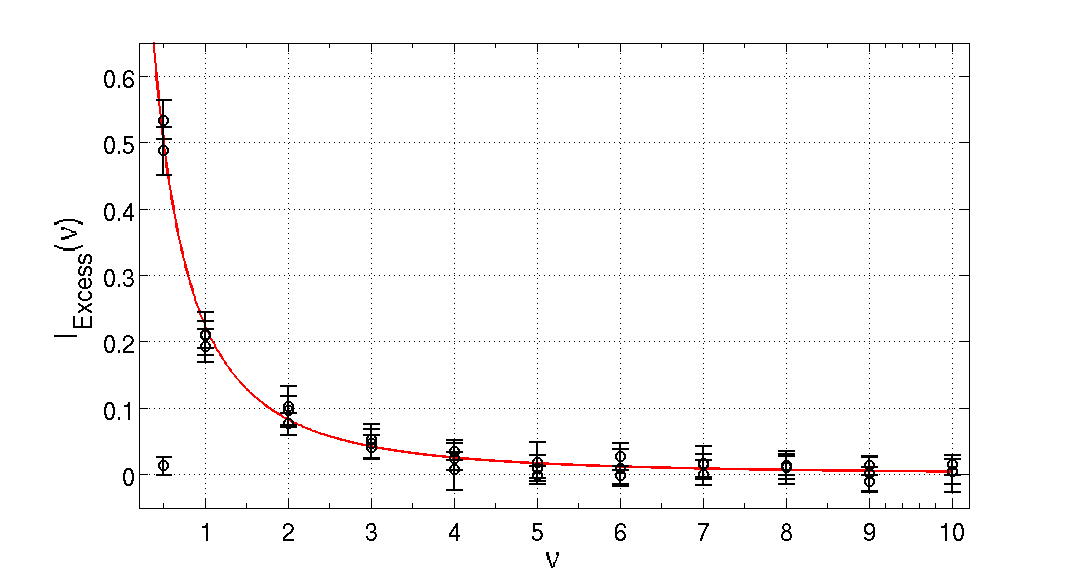
\includegraphics[width =\textwidth]{./figuras/I_Excess.png} 
 \caption[Excesso de informação mútua na cópula \textit{t}]{Excesso de informação mútua na cópula \textit{t}. $I(\nu)$, como dado na eq.\eqref{eq:excesst}. Círculos mostram estimativas para 20 amostragens de pontos de uma cópula \textit{t} usando o método de ``moment matching'' para diversos valores de correlação e $\nu$.}
 \label{fig:ajuste}
\end{figure}
\section{Conclusões}

\newthought{A literatura em teoria de informação e teoria de cópulas e dependência estatística} - ambas com décadas de existência - se desenvolveram em relativo isolamento, com apenas pontos muito recentes de contato. Neste trabalho tentamos discutir as consequencias de alguns desses pontos e conexões entre os dois tópicos. A teoria de cópulas pode ser usada para decompor as distribuições conjuntas em flutuações idiossincráticas das marginais de cada variável e flutuações devidas ao acoplamento entre as variáveis. A conexão com a teoria de informação permite levar adiante essa decomposição e isolar contribuições à informação total contida na distribuição em partes relativas às marginais, ao acoplamento de natureza linear e acoplamentos de mais alta ordem. Essa decomposição oferece testes simples a respeito da linearidade e ``gaussianidade'' do acoplamento e também sugere um método de ajuste de cópulas baseados no ajuste da informação mútua. Essa abordagem também clarifica os perigos do uso da correlação linear como medida de dependência em séries financeiras para, por exemplo, estimativas de riscos de contratos complexos e otimização de carteiras, pois essa medida é fadada a subestimar a dependência em séries em que flutuações não-gaussianas são esperadas. Finalmente, pensamos que uma conexão entre essas duas áreas - teoria de informação e teoria de dependência estatística - pode ser útil em fornecer conceitos e técnicas novas para o estudo de sistemas complexos. 
